

	\documentclass[10pt,parskip=half,
	toc=sectionentrywithdots,
	bibliography=totocnumbered,
	captions=tableheading,numbers=noendperiod]{scrartcl}

    \usepackage[T1]{fontenc} % Nicer default font (+ math font) than Computer Modern for most use cases
    \usepackage{mathpazo}
    \usepackage{graphicx}
    \usepackage[skip=3pt]{caption}
    \usepackage{adjustbox} % Used to constrain images to a maximum size
    \usepackage[table]{xcolor} % Allow colors to be defined
    \usepackage{enumerate} % Needed for markdown enumerations to work
    \usepackage{amsmath} % Equations
    \usepackage{amssymb} % Equations
    \usepackage{textcomp} % defines textquotesingle
    % Hack from http://tex.stackexchange.com/a/47451/13684:
    \AtBeginDocument{%
        \def\PYZsq{\textquotesingle}% Upright quotes in Pygmentized code
    }
    \usepackage{upquote} % Upright quotes for verbatim code
    \usepackage{eurosym} % defines \euro
    \usepackage[mathletters]{ucs} % Extended unicode (utf-8) support
    \usepackage[utf8x]{inputenc} % Allow utf-8 characters in the tex document
    \usepackage{fancyvrb} % verbatim replacement that allows latex
    \usepackage{grffile} % extends the file name processing of package graphics
                         % to support a larger range
    % The hyperref package gives us a pdf with properly built
    % internal navigation ('pdf bookmarks' for the table of contents,
    % internal cross-reference links, web links for URLs, etc.)
    \usepackage{hyperref}
    \usepackage{longtable} % longtable support required by pandoc >1.10
    \usepackage{booktabs}  % table support for pandoc > 1.12.2
    \usepackage[inline]{enumitem} % IRkernel/repr support (it uses the enumerate* environment)
    \usepackage[normalem]{ulem} % ulem is needed to support strikethroughs (\sout)
                                % normalem makes italics be italics, not underlines

    \usepackage{translations}
	\usepackage{microtype} % improves the spacing between words and letters
	\usepackage{placeins} % placement of figures
    % could use \usepackage[section]{placeins} but placing in subsection in command section
	% Places the float at precisely the location in the LaTeX code (with H)
	\usepackage{float}
	\usepackage[colorinlistoftodos,obeyFinal,textwidth=.8in]{todonotes} % to mark to-dos
	% number figures, tables and equations by section
	\usepackage{chngcntr}
	% header/footer
	\usepackage[footsepline=0.25pt]{scrlayer-scrpage}

	% bibliography formatting
	\usepackage[numbers, square, super, sort&compress]{natbib}
	% hyperlink doi's
	\usepackage{doi}

    % define a code float
    \usepackage{newfloat} % to define a new float types
    \DeclareFloatingEnvironment[
        fileext=frm,placement={!ht},
        within=section,name=Code]{codecell}
    \DeclareFloatingEnvironment[
        fileext=frm,placement={!ht},
        within=section,name=Text]{textcell}
    \DeclareFloatingEnvironment[
        fileext=frm,placement={!ht},
        within=section,name=Text]{errorcell}

    \usepackage{listings} % a package for wrapping code in a box
    \usepackage[framemethod=tikz]{mdframed} % to fram code

% Pygments definitions

\makeatletter
\def\PY@reset{\let\PY@it=\relax \let\PY@bf=\relax%
    \let\PY@ul=\relax \let\PY@tc=\relax%
    \let\PY@bc=\relax \let\PY@ff=\relax}
\def\PY@tok#1{\csname PY@tok@#1\endcsname}
\def\PY@toks#1+{\ifx\relax#1\empty\else%
    \PY@tok{#1}\expandafter\PY@toks\fi}
\def\PY@do#1{\PY@bc{\PY@tc{\PY@ul{%
    \PY@it{\PY@bf{\PY@ff{#1}}}}}}}
\def\PY#1#2{\PY@reset\PY@toks#1+\relax+\PY@do{#2}}

\expandafter\def\csname PY@tok@w\endcsname{\def\PY@tc##1{\textcolor[rgb]{0.73,0.73,0.73}{##1}}}
\expandafter\def\csname PY@tok@c\endcsname{\let\PY@it=\textit\def\PY@tc##1{\textcolor[rgb]{0.25,0.50,0.50}{##1}}}
\expandafter\def\csname PY@tok@cp\endcsname{\def\PY@tc##1{\textcolor[rgb]{0.74,0.48,0.00}{##1}}}
\expandafter\def\csname PY@tok@k\endcsname{\let\PY@bf=\textbf\def\PY@tc##1{\textcolor[rgb]{0.00,0.50,0.00}{##1}}}
\expandafter\def\csname PY@tok@kp\endcsname{\def\PY@tc##1{\textcolor[rgb]{0.00,0.50,0.00}{##1}}}
\expandafter\def\csname PY@tok@kt\endcsname{\def\PY@tc##1{\textcolor[rgb]{0.69,0.00,0.25}{##1}}}
\expandafter\def\csname PY@tok@o\endcsname{\def\PY@tc##1{\textcolor[rgb]{0.40,0.40,0.40}{##1}}}
\expandafter\def\csname PY@tok@ow\endcsname{\let\PY@bf=\textbf\def\PY@tc##1{\textcolor[rgb]{0.67,0.13,1.00}{##1}}}
\expandafter\def\csname PY@tok@nb\endcsname{\def\PY@tc##1{\textcolor[rgb]{0.00,0.50,0.00}{##1}}}
\expandafter\def\csname PY@tok@nf\endcsname{\def\PY@tc##1{\textcolor[rgb]{0.00,0.00,1.00}{##1}}}
\expandafter\def\csname PY@tok@nc\endcsname{\let\PY@bf=\textbf\def\PY@tc##1{\textcolor[rgb]{0.00,0.00,1.00}{##1}}}
\expandafter\def\csname PY@tok@nn\endcsname{\let\PY@bf=\textbf\def\PY@tc##1{\textcolor[rgb]{0.00,0.00,1.00}{##1}}}
\expandafter\def\csname PY@tok@ne\endcsname{\let\PY@bf=\textbf\def\PY@tc##1{\textcolor[rgb]{0.82,0.25,0.23}{##1}}}
\expandafter\def\csname PY@tok@nv\endcsname{\def\PY@tc##1{\textcolor[rgb]{0.10,0.09,0.49}{##1}}}
\expandafter\def\csname PY@tok@no\endcsname{\def\PY@tc##1{\textcolor[rgb]{0.53,0.00,0.00}{##1}}}
\expandafter\def\csname PY@tok@nl\endcsname{\def\PY@tc##1{\textcolor[rgb]{0.63,0.63,0.00}{##1}}}
\expandafter\def\csname PY@tok@ni\endcsname{\let\PY@bf=\textbf\def\PY@tc##1{\textcolor[rgb]{0.60,0.60,0.60}{##1}}}
\expandafter\def\csname PY@tok@na\endcsname{\def\PY@tc##1{\textcolor[rgb]{0.49,0.56,0.16}{##1}}}
\expandafter\def\csname PY@tok@nt\endcsname{\let\PY@bf=\textbf\def\PY@tc##1{\textcolor[rgb]{0.00,0.50,0.00}{##1}}}
\expandafter\def\csname PY@tok@nd\endcsname{\def\PY@tc##1{\textcolor[rgb]{0.67,0.13,1.00}{##1}}}
\expandafter\def\csname PY@tok@s\endcsname{\def\PY@tc##1{\textcolor[rgb]{0.73,0.13,0.13}{##1}}}
\expandafter\def\csname PY@tok@sd\endcsname{\let\PY@it=\textit\def\PY@tc##1{\textcolor[rgb]{0.73,0.13,0.13}{##1}}}
\expandafter\def\csname PY@tok@si\endcsname{\let\PY@bf=\textbf\def\PY@tc##1{\textcolor[rgb]{0.73,0.40,0.53}{##1}}}
\expandafter\def\csname PY@tok@se\endcsname{\let\PY@bf=\textbf\def\PY@tc##1{\textcolor[rgb]{0.73,0.40,0.13}{##1}}}
\expandafter\def\csname PY@tok@sr\endcsname{\def\PY@tc##1{\textcolor[rgb]{0.73,0.40,0.53}{##1}}}
\expandafter\def\csname PY@tok@ss\endcsname{\def\PY@tc##1{\textcolor[rgb]{0.10,0.09,0.49}{##1}}}
\expandafter\def\csname PY@tok@sx\endcsname{\def\PY@tc##1{\textcolor[rgb]{0.00,0.50,0.00}{##1}}}
\expandafter\def\csname PY@tok@m\endcsname{\def\PY@tc##1{\textcolor[rgb]{0.40,0.40,0.40}{##1}}}
\expandafter\def\csname PY@tok@gh\endcsname{\let\PY@bf=\textbf\def\PY@tc##1{\textcolor[rgb]{0.00,0.00,0.50}{##1}}}
\expandafter\def\csname PY@tok@gu\endcsname{\let\PY@bf=\textbf\def\PY@tc##1{\textcolor[rgb]{0.50,0.00,0.50}{##1}}}
\expandafter\def\csname PY@tok@gd\endcsname{\def\PY@tc##1{\textcolor[rgb]{0.63,0.00,0.00}{##1}}}
\expandafter\def\csname PY@tok@gi\endcsname{\def\PY@tc##1{\textcolor[rgb]{0.00,0.63,0.00}{##1}}}
\expandafter\def\csname PY@tok@gr\endcsname{\def\PY@tc##1{\textcolor[rgb]{1.00,0.00,0.00}{##1}}}
\expandafter\def\csname PY@tok@ge\endcsname{\let\PY@it=\textit}
\expandafter\def\csname PY@tok@gs\endcsname{\let\PY@bf=\textbf}
\expandafter\def\csname PY@tok@gp\endcsname{\let\PY@bf=\textbf\def\PY@tc##1{\textcolor[rgb]{0.00,0.00,0.50}{##1}}}
\expandafter\def\csname PY@tok@go\endcsname{\def\PY@tc##1{\textcolor[rgb]{0.53,0.53,0.53}{##1}}}
\expandafter\def\csname PY@tok@gt\endcsname{\def\PY@tc##1{\textcolor[rgb]{0.00,0.27,0.87}{##1}}}
\expandafter\def\csname PY@tok@err\endcsname{\def\PY@bc##1{\setlength{\fboxsep}{0pt}\fcolorbox[rgb]{1.00,0.00,0.00}{1,1,1}{\strut ##1}}}
\expandafter\def\csname PY@tok@kc\endcsname{\let\PY@bf=\textbf\def\PY@tc##1{\textcolor[rgb]{0.00,0.50,0.00}{##1}}}
\expandafter\def\csname PY@tok@kd\endcsname{\let\PY@bf=\textbf\def\PY@tc##1{\textcolor[rgb]{0.00,0.50,0.00}{##1}}}
\expandafter\def\csname PY@tok@kn\endcsname{\let\PY@bf=\textbf\def\PY@tc##1{\textcolor[rgb]{0.00,0.50,0.00}{##1}}}
\expandafter\def\csname PY@tok@kr\endcsname{\let\PY@bf=\textbf\def\PY@tc##1{\textcolor[rgb]{0.00,0.50,0.00}{##1}}}
\expandafter\def\csname PY@tok@bp\endcsname{\def\PY@tc##1{\textcolor[rgb]{0.00,0.50,0.00}{##1}}}
\expandafter\def\csname PY@tok@fm\endcsname{\def\PY@tc##1{\textcolor[rgb]{0.00,0.00,1.00}{##1}}}
\expandafter\def\csname PY@tok@vc\endcsname{\def\PY@tc##1{\textcolor[rgb]{0.10,0.09,0.49}{##1}}}
\expandafter\def\csname PY@tok@vg\endcsname{\def\PY@tc##1{\textcolor[rgb]{0.10,0.09,0.49}{##1}}}
\expandafter\def\csname PY@tok@vi\endcsname{\def\PY@tc##1{\textcolor[rgb]{0.10,0.09,0.49}{##1}}}
\expandafter\def\csname PY@tok@vm\endcsname{\def\PY@tc##1{\textcolor[rgb]{0.10,0.09,0.49}{##1}}}
\expandafter\def\csname PY@tok@sa\endcsname{\def\PY@tc##1{\textcolor[rgb]{0.73,0.13,0.13}{##1}}}
\expandafter\def\csname PY@tok@sb\endcsname{\def\PY@tc##1{\textcolor[rgb]{0.73,0.13,0.13}{##1}}}
\expandafter\def\csname PY@tok@sc\endcsname{\def\PY@tc##1{\textcolor[rgb]{0.73,0.13,0.13}{##1}}}
\expandafter\def\csname PY@tok@dl\endcsname{\def\PY@tc##1{\textcolor[rgb]{0.73,0.13,0.13}{##1}}}
\expandafter\def\csname PY@tok@s2\endcsname{\def\PY@tc##1{\textcolor[rgb]{0.73,0.13,0.13}{##1}}}
\expandafter\def\csname PY@tok@sh\endcsname{\def\PY@tc##1{\textcolor[rgb]{0.73,0.13,0.13}{##1}}}
\expandafter\def\csname PY@tok@s1\endcsname{\def\PY@tc##1{\textcolor[rgb]{0.73,0.13,0.13}{##1}}}
\expandafter\def\csname PY@tok@mb\endcsname{\def\PY@tc##1{\textcolor[rgb]{0.40,0.40,0.40}{##1}}}
\expandafter\def\csname PY@tok@mf\endcsname{\def\PY@tc##1{\textcolor[rgb]{0.40,0.40,0.40}{##1}}}
\expandafter\def\csname PY@tok@mh\endcsname{\def\PY@tc##1{\textcolor[rgb]{0.40,0.40,0.40}{##1}}}
\expandafter\def\csname PY@tok@mi\endcsname{\def\PY@tc##1{\textcolor[rgb]{0.40,0.40,0.40}{##1}}}
\expandafter\def\csname PY@tok@il\endcsname{\def\PY@tc##1{\textcolor[rgb]{0.40,0.40,0.40}{##1}}}
\expandafter\def\csname PY@tok@mo\endcsname{\def\PY@tc##1{\textcolor[rgb]{0.40,0.40,0.40}{##1}}}
\expandafter\def\csname PY@tok@ch\endcsname{\let\PY@it=\textit\def\PY@tc##1{\textcolor[rgb]{0.25,0.50,0.50}{##1}}}
\expandafter\def\csname PY@tok@cm\endcsname{\let\PY@it=\textit\def\PY@tc##1{\textcolor[rgb]{0.25,0.50,0.50}{##1}}}
\expandafter\def\csname PY@tok@cpf\endcsname{\let\PY@it=\textit\def\PY@tc##1{\textcolor[rgb]{0.25,0.50,0.50}{##1}}}
\expandafter\def\csname PY@tok@c1\endcsname{\let\PY@it=\textit\def\PY@tc##1{\textcolor[rgb]{0.25,0.50,0.50}{##1}}}
\expandafter\def\csname PY@tok@cs\endcsname{\let\PY@it=\textit\def\PY@tc##1{\textcolor[rgb]{0.25,0.50,0.50}{##1}}}

\def\PYZbs{\char`\\}
\def\PYZus{\char`\_}
\def\PYZob{\char`\{}
\def\PYZcb{\char`\}}
\def\PYZca{\char`\^}
\def\PYZam{\char`\&}
\def\PYZlt{\char`\<}
\def\PYZgt{\char`\>}
\def\PYZsh{\char`\#}
\def\PYZpc{\char`\%}
\def\PYZdl{\char`\$}
\def\PYZhy{\char`\-}
\def\PYZsq{\char`\'}
\def\PYZdq{\char`\"}
\def\PYZti{\char`\~}
% for compatibility with earlier versions
\def\PYZat{@}
\def\PYZlb{[}
\def\PYZrb{]}
\makeatother

% ANSI colors
\definecolor{ansi-black}{HTML}{3E424D}
\definecolor{ansi-black-intense}{HTML}{282C36}
\definecolor{ansi-red}{HTML}{E75C58}
\definecolor{ansi-red-intense}{HTML}{B22B31}
\definecolor{ansi-green}{HTML}{00A250}
\definecolor{ansi-green-intense}{HTML}{007427}
\definecolor{ansi-yellow}{HTML}{DDB62B}
\definecolor{ansi-yellow-intense}{HTML}{B27D12}
\definecolor{ansi-blue}{HTML}{208FFB}
\definecolor{ansi-blue-intense}{HTML}{0065CA}
\definecolor{ansi-magenta}{HTML}{D160C4}
\definecolor{ansi-magenta-intense}{HTML}{A03196}
\definecolor{ansi-cyan}{HTML}{60C6C8}
\definecolor{ansi-cyan-intense}{HTML}{258F8F}
\definecolor{ansi-white}{HTML}{C5C1B4}
\definecolor{ansi-white-intense}{HTML}{A1A6B2}

% commands and environments needed by pandoc snippets
% extracted from the output of `pandoc -s`
\providecommand{\tightlist}{%
  \setlength{\itemsep}{0pt}\setlength{\parskip}{0pt}}
\DefineVerbatimEnvironment{Highlighting}{Verbatim}{commandchars=\\\{\}}
% Add ',fontsize=\small' for more characters per line
\newenvironment{Shaded}{}{}
\newcommand{\KeywordTok}[1]{\textcolor[rgb]{0.00,0.44,0.13}{\textbf{{#1}}}}
\newcommand{\DataTypeTok}[1]{\textcolor[rgb]{0.56,0.13,0.00}{{#1}}}
\newcommand{\DecValTok}[1]{\textcolor[rgb]{0.25,0.63,0.44}{{#1}}}
\newcommand{\BaseNTok}[1]{\textcolor[rgb]{0.25,0.63,0.44}{{#1}}}
\newcommand{\FloatTok}[1]{\textcolor[rgb]{0.25,0.63,0.44}{{#1}}}
\newcommand{\CharTok}[1]{\textcolor[rgb]{0.25,0.44,0.63}{{#1}}}
\newcommand{\StringTok}[1]{\textcolor[rgb]{0.25,0.44,0.63}{{#1}}}
\newcommand{\CommentTok}[1]{\textcolor[rgb]{0.38,0.63,0.69}{\textit{{#1}}}}
\newcommand{\OtherTok}[1]{\textcolor[rgb]{0.00,0.44,0.13}{{#1}}}
\newcommand{\AlertTok}[1]{\textcolor[rgb]{1.00,0.00,0.00}{\textbf{{#1}}}}
\newcommand{\FunctionTok}[1]{\textcolor[rgb]{0.02,0.16,0.49}{{#1}}}
\newcommand{\RegionMarkerTok}[1]{{#1}}
\newcommand{\ErrorTok}[1]{\textcolor[rgb]{1.00,0.00,0.00}{\textbf{{#1}}}}
\newcommand{\NormalTok}[1]{{#1}}

% Additional commands for more recent versions of Pandoc
\newcommand{\ConstantTok}[1]{\textcolor[rgb]{0.53,0.00,0.00}{{#1}}}
\newcommand{\SpecialCharTok}[1]{\textcolor[rgb]{0.25,0.44,0.63}{{#1}}}
\newcommand{\VerbatimStringTok}[1]{\textcolor[rgb]{0.25,0.44,0.63}{{#1}}}
\newcommand{\SpecialStringTok}[1]{\textcolor[rgb]{0.73,0.40,0.53}{{#1}}}
\newcommand{\ImportTok}[1]{{#1}}
\newcommand{\DocumentationTok}[1]{\textcolor[rgb]{0.73,0.13,0.13}{\textit{{#1}}}}
\newcommand{\AnnotationTok}[1]{\textcolor[rgb]{0.38,0.63,0.69}{\textbf{\textit{{#1}}}}}
\newcommand{\CommentVarTok}[1]{\textcolor[rgb]{0.38,0.63,0.69}{\textbf{\textit{{#1}}}}}
\newcommand{\VariableTok}[1]{\textcolor[rgb]{0.10,0.09,0.49}{{#1}}}
\newcommand{\ControlFlowTok}[1]{\textcolor[rgb]{0.00,0.44,0.13}{\textbf{{#1}}}}
\newcommand{\OperatorTok}[1]{\textcolor[rgb]{0.40,0.40,0.40}{{#1}}}
\newcommand{\BuiltInTok}[1]{{#1}}
\newcommand{\ExtensionTok}[1]{{#1}}
\newcommand{\PreprocessorTok}[1]{\textcolor[rgb]{0.74,0.48,0.00}{{#1}}}
\newcommand{\AttributeTok}[1]{\textcolor[rgb]{0.49,0.56,0.16}{{#1}}}
\newcommand{\InformationTok}[1]{\textcolor[rgb]{0.38,0.63,0.69}{\textbf{\textit{{#1}}}}}
\newcommand{\WarningTok}[1]{\textcolor[rgb]{0.38,0.63,0.69}{\textbf{\textit{{#1}}}}}

% Define a nice break command that doesn't care if a line doesn't already
% exist.
\def\br{\hspace*{\fill} \\* }

% Math Jax compatability definitions
\def\gt{>}
\def\lt{<}

    \setcounter{secnumdepth}{5}

    % Colors for the hyperref package
    \definecolor{urlcolor}{rgb}{0,.145,.698}
    \definecolor{linkcolor}{rgb}{.71,0.21,0.01}
    \definecolor{citecolor}{rgb}{.12,.54,.11}

\DeclareTranslationFallback{Author}{Author}
\DeclareTranslation{Portuges}{Author}{Autor}

\DeclareTranslationFallback{List of Codes}{List of Codes}
\DeclareTranslation{Catalan}{List of Codes}{Llista de Codis}
\DeclareTranslation{Danish}{List of Codes}{Liste over Koder}
\DeclareTranslation{German}{List of Codes}{Liste der Codes}
\DeclareTranslation{Spanish}{List of Codes}{Lista de C\'{o}digos}
\DeclareTranslation{French}{List of Codes}{Liste des Codes}
\DeclareTranslation{Italian}{List of Codes}{Elenco dei Codici}
\DeclareTranslation{Dutch}{List of Codes}{Lijst van Codes}
\DeclareTranslation{Portuges}{List of Codes}{Lista de C\'{o}digos}

\DeclareTranslationFallback{Supervisors}{Supervisors}
\DeclareTranslation{Catalan}{Supervisors}{Supervisors}
\DeclareTranslation{Danish}{Supervisors}{Vejledere}
\DeclareTranslation{German}{Supervisors}{Vorgesetzten}
\DeclareTranslation{Spanish}{Supervisors}{Supervisores}
\DeclareTranslation{French}{Supervisors}{Superviseurs}
\DeclareTranslation{Italian}{Supervisors}{Le autorit\`{a} di vigilanza}
\DeclareTranslation{Dutch}{Supervisors}{supervisors}
\DeclareTranslation{Portuguese}{Supervisors}{Supervisores}

\definecolor{codegreen}{rgb}{0,0.6,0}
\definecolor{codegray}{rgb}{0.5,0.5,0.5}
\definecolor{codepurple}{rgb}{0.58,0,0.82}
\definecolor{backcolour}{rgb}{0.95,0.95,0.95}

\lstdefinestyle{mystyle}{
    commentstyle=\color{codegreen},
    keywordstyle=\color{magenta},
    numberstyle=\tiny\color{codegray},
    stringstyle=\color{codepurple},
    basicstyle=\ttfamily,
    breakatwhitespace=false,
    keepspaces=true,
    numbers=left,
    numbersep=10pt,
    showspaces=false,
    showstringspaces=false,
    showtabs=false,
    tabsize=2,
    breaklines=true,
    literate={\-}{}{0\discretionary{-}{}{-}},
  postbreak=\mbox{\textcolor{red}{$\hookrightarrow$}\space},
}

\lstset{style=mystyle}

\surroundwithmdframed[
  hidealllines=true,
  backgroundcolor=backcolour,
  innerleftmargin=0pt,
  innerrightmargin=0pt,
  innertopmargin=0pt,
  innerbottommargin=0pt]{lstlisting}

 % Used to adjust the document margins
\usepackage{geometry}
\geometry{tmargin=1in,bmargin=1in,lmargin=1in,rmargin=1in,
nohead,includefoot,footskip=25pt}
% you can use showframe option to check the margins visually

	% ensure new section starts on new page
	\addtokomafont{section}{\clearpage}

    % Prevent overflowing lines due to hard-to-break entities
    \sloppy

    % Setup hyperref package
    \hypersetup{
      breaklinks=true,  % so long urls are correctly broken across lines
      colorlinks=true,
      urlcolor=urlcolor,
      linkcolor=linkcolor,
      citecolor=citecolor,
      }

    % ensure figures are placed within subsections
    \makeatletter
    \AtBeginDocument{%
      \expandafter\renewcommand\expandafter\subsection\expandafter
        {\expandafter\@fb@secFB\subsection}%
      \newcommand\@fb@secFB{\FloatBarrier
        \gdef\@fb@afterHHook{\@fb@topbarrier \gdef\@fb@afterHHook{}}}%
      \g@addto@macro\@afterheading{\@fb@afterHHook}%
      \gdef\@fb@afterHHook{}%
    }
    \makeatother

	% number figures, tables and equations by section
	\usepackage{chngcntr}
	\counterwithout{figure}{section}
	\counterwithout{table}{section}
	\counterwithout{equation}{section}
	\makeatletter
	\@addtoreset{table}{section}
	\@addtoreset{figure}{section}
	\@addtoreset{equation}{section}
	\makeatother
	\renewcommand\thetable{\thesection.\arabic{table}}
	\renewcommand\thefigure{\thesection.\arabic{figure}}
	\renewcommand\theequation{\thesection.\arabic{equation}}

        % set global options for float placement
        \makeatletter
          \providecommand*\setfloatlocations[2]{\@namedef{fps@#1}{#2}}
        \makeatother

    % align captions to left (indented)
	\captionsetup{justification=raggedright,
	singlelinecheck=false,format=hang,labelfont={it,bf}}

	% shift footer down so space between separation line
	\ModifyLayer[addvoffset=.6ex]{scrheadings.foot.odd}
	\ModifyLayer[addvoffset=.6ex]{scrheadings.foot.even}
	\ModifyLayer[addvoffset=.6ex]{scrheadings.foot.oneside}
	\ModifyLayer[addvoffset=.6ex]{plain.scrheadings.foot.odd}
	\ModifyLayer[addvoffset=.6ex]{plain.scrheadings.foot.even}
	\ModifyLayer[addvoffset=.6ex]{plain.scrheadings.foot.oneside}
	\pagestyle{scrheadings}
	\clearscrheadfoot{}
	\ifoot{\leftmark}
	\renewcommand{\sectionmark}[1]{\markleft{\thesection\ #1}}
	\ofoot{\pagemark}
	\cfoot{}

% clereref must be loaded after anything that changes the referencing system
\usepackage{cleveref}
\creflabelformat{equation}{#2#1#3}

% make the code float work with cleverref
\crefname{codecell}{code}{codes}
\Crefname{codecell}{code}{codes}
% make the text float work with cleverref
\crefname{textcell}{text}{texts}
\Crefname{textcell}{text}{texts}
% make the text float work with cleverref
\crefname{errorcell}{error}{errors}
\Crefname{errorcell}{error}{errors}

	\begin{document}

		\begin{titlepage}
	\begin{flushright}
		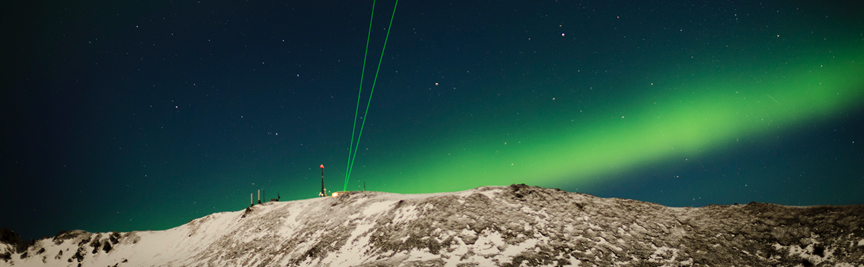
\includegraphics[width=0.7\textwidth]{report_example_files/NEGI2018.png}
	\end{flushright}

	\begin{center}

	\vspace*{1cm}

	\Huge\textbf{Climate science at high latitudes: Modeling and model evaluation}

	\vspace{0.5cm}\LARGE{Example for writing your report}

	\vspace{1.5cm}

	\begin{minipage}{0.8\textwidth}
		\begin{center}
		\begin{minipage}{0.39\textwidth}
		\begin{flushleft} \Large
		\emph{\GetTranslation{Author}:}\\Anne Fouilloux\\\href{mailto:authors@email.com}{authors@email.com}
		\end{flushleft}
		\end{minipage}
		\hspace{\fill}
		\begin{minipage}{0.39\textwidth}
		\begin{flushright} \Large\emph{\GetTranslation{Supervisors}:} \\
			  First Supervisor
			  Second Supervisor
		\end{flushright}
		\end{minipage}
		\end{center}
	\end{minipage}

	\vfill

	\begin{minipage}{0.8\textwidth}
	\begin{center}\LARGE{A tagline for the report.}
	\end{center}
	\end{minipage}

	\vspace{0.8cm}
		  \LARGE{Institution1}\\
		  \LARGE{Institution2}\\

	\vspace{0.4cm}

	\today

	\end{center}
	\end{titlepage}

		\begingroup
    \let\cleardoublepage\relax
    \let\clearpage\relax\tableofcontents\listoffigures\listoftables\listof{codecell}{\GetTranslation{List of Codes}}
    \endgroup

\section{General structure}\label{general-structure}

\begin{itemize}
\tightlist
\item
  Project title
\item
  Name, email, course title, date, group assistant
\item
  Abstract (1/2 page max)
\item
  Introduction (1 page)
\item
  Method

  \begin{itemize}
  \tightlist
  \item
    Packages used
  \item
    Datasets (models and observations)
  \item
    Analysis method
  \item
    \ldots{}
  \end{itemize}
\item
  Results
\item
  Discussion and outlook (1 page)
\item
  Conclusions (1/2 page)
\item
  References
\item
  Acknowledgments
\end{itemize}

\section{How to generate pdf report}\label{how-to-generate-pdf-report}

\subsection{Markdown}\label{markdown}

\begin{itemize}
\tightlist
\item
  Select Markdown cell instead of code cell
\item
  \href{https://github.com/adam-p/markdown-here/wiki/Markdown-Cheatsheet}{Markdown
  cheatsheet}
\end{itemize}

\subsection{Add a report title}\label{add-a-report-title}

\begin{itemize}
\tightlist
\item
  Edit -\/-\textgreater{} Edit Notebook Metadata
\end{itemize}

\begin{Shaded}
\begin{Highlighting}[]
 \StringTok{"ipub"}\NormalTok{: }\KeywordTok{\{}
    \StringTok{"bibliography"}\NormalTok{: }\StringTok{"/mnt/data/teachers/annefou/test_report.bib"}\NormalTok{,}
    \StringTok{"titlepage"}\NormalTok{: }\KeywordTok{\{}
      \StringTok{"author"}\NormalTok{: }\StringTok{"Anne Fouilloux"}\NormalTok{,}
      \StringTok{"email"}\NormalTok{: }\StringTok{"authors@email.com"}\NormalTok{,}
      \StringTok{"institution"}\NormalTok{:}\BuiltInTok{ [}
        \StringTok{"Institution1"}\NormalTok{,}
        \StringTok{"Institution2"}
\NormalTok{      ],}
      \StringTok{"logo"}\NormalTok{: }\StringTok{"/mnt/data/teachers/annefou/NEGI2018.png"}\NormalTok{,}
      \StringTok{"subtitle"}\NormalTok{: }\StringTok{"Example for writing your report"}\NormalTok{,}
      \StringTok{"supervisors"}\NormalTok{: [}
        \StringTok{"First Supervisor"}\NormalTok{,}
        \StringTok{"Second Supervisor"}
\NormalTok{      ],}
      \StringTok{"tagline"}\NormalTok{: }\StringTok{"A tagline for the report."}\NormalTok{,}
      \StringTok{"title"}\NormalTok{: }\StringTok{"Climate science at high latitudes: Modeling and model evaluation"}
\NormalTok{    \}}
\NormalTok{  \},}
\end{Highlighting}
\end{Shaded}

\subsection{Hide a cell output}\label{hide-a-cell-output}

View -\/-\textgreater{} Cell Toolbar -\/-\textgreater{} Edit Metadata

And add:

\begin{Shaded}
\begin{Highlighting}[]
  \StringTok{"ipub"}\NormalTok{: }\KeywordTok{\{}
    \StringTok{"ignore"}\NormalTok{: }\FunctionTok{true}
  \KeywordTok{\}}
\end{Highlighting}
\end{Shaded}

\subsection{Add Code block}\label{add-code-block}

In the Cell metadata:

\begin{Shaded}
\begin{Highlighting}[]
\StringTok{"ipub"}\NormalTok{: }\KeywordTok{\{}
  \StringTok{"code"}\NormalTok{: }\KeywordTok{\{}
    \StringTok{"format"} \BuiltInTok{:} \DataTypeTok{\{\}}\NormalTok{,}
    \StringTok{"asfloat"}\NormalTok{: }\FunctionTok{true}\NormalTok{,}
    \StringTok{"caption"}\NormalTok{: }\StringTok{""}\NormalTok{,}
    \StringTok{"label"}\NormalTok{: }\StringTok{"code:example_code"}\NormalTok{,}
    \StringTok{"widefigure"}\NormalTok{: }\FunctionTok{false}\NormalTok{,}
    \StringTok{"placement"}\NormalTok{: }\StringTok{"H"}
    \KeywordTok{\}}
  \KeywordTok{\}}
\end{Highlighting}
\end{Shaded}

\subsection{Add a latex reference}\label{add-a-latex-reference}

\subsubsection{Figures}\label{figures}

There are two ways to reference plots:

\begin{enumerate}
\def\labelenumi{\arabic{enumi}.}
\tightlist
\item
  Use latex syntax:
\end{enumerate}

\begin{itemize}
\tightlist
\item
  Save your figure in a code cell:
\end{itemize}

\begin{Shaded}
\begin{Highlighting}[]
\NormalTok{fig.savefig(}\StringTok{'fig_example.png'}\NormalTok{) }\OperatorTok{;}
\end{Highlighting}
\end{Shaded}

where fig is a matplotlib figure (fig = plt.figure ( figsize ={[}12
,5{]})).

\begin{itemize}
\tightlist
\item
  Reference your plot in a markdown cell:
\end{itemize}

In both cases, you can reference your plots using latex syntax
\texttt{\textbackslash{}ref}

\subsubsection{cite a paper}\label{cite-a-paper}

For all the paper in your bib file (added in the notebook metadata), you
can use the following syntax to cite your paper:

\begin{itemize}
\tightlist
\item
  you can add a citation using latex citation
  \texttt{\textbackslash{}cite}.
\end{itemize}

\subsection{Generate pdf with
nbpublish}\label{generate-pdf-with-nbpublish}

To convert your jupyter notebook into pdf, you need to use nbpublish.
See last cell of this jupyter notebook.

\begin{Shaded}
\begin{Highlighting}[]
\NormalTok{!}\ExtensionTok{nbpublish}\NormalTok{ -f latex_ipypublish_all -pdf report_example.ipynb}
\end{Highlighting}
\end{Shaded}

\section{Import python packages}\label{import-python-packages}

\begin{lstlisting}[language=Python,numbers=left,xleftmargin=20pt,xrightmargin=5pt,belowskip=5pt,aboveskip=5pt]
import xarray as xr
import dask . array as da
import matplotlib . pyplot as plt
import cartopy.crs as ccrs
import numpy as np
import pandas as pd
%matplotlib inline

\end{lstlisting}

\section{Data and Methods}\label{data-and-methods}

\subsection{Read Data}\label{read-data}

\begin{lstlisting}[language=Python,numbers=left,xleftmargin=20pt,xrightmargin=5pt,belowskip=5pt,aboveskip=5pt]
dset = xr.open_dataset('/mnt/data/students/evelien/Observations/air.mon.mean.seasonal.arctic.nc')
\end{lstlisting}

\begin{lstlisting}[language=Python,numbers=left,xleftmargin=20pt,xrightmargin=5pt,belowskip=5pt,aboveskip=5pt]
dset . time
\end{lstlisting}

\begin{lstlisting}[language={},postbreak={},numbers=none,xrightmargin=7pt,breakindent=0pt,aboveskip=5pt,belowskip=5pt]
<xarray.DataArray 'time' (time: 461)>
array(['1900-01-16T12:00:00.000000000', '1900-04-01T00:00:00.000000000',
       '1900-07-01T00:00:00.000000000', ..., '2014-07-01T00:00:00.000000000',
       '2014-10-01T00:00:00.000000000', '2014-12-01T00:00:00.000000000'],
      dtype='datetime64[ns]')
Coordinates:
  * time     (time) datetime64[ns] 1900-01-16T12:00:00 1900-04-01 ... 2014-12-01
Attributes:
    standard_name:  time
    long_name:      Time
    bounds:         time_bnds
    axis:           T
\end{lstlisting}

\subsubsection{Select the nearest date}\label{select-the-nearest-date}

\begin{lstlisting}[language=Python,numbers=left,xleftmargin=20pt,xrightmargin=5pt,belowskip=5pt,aboveskip=5pt]
x = dset["air"].sel( time ="1989-01-01T00:00:00.000000000", method = 'nearest')

\end{lstlisting}

\section{Results}\label{results}

\begin{figure}
  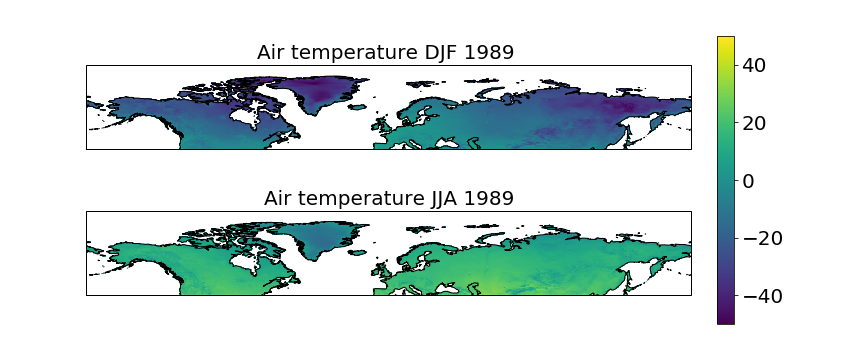
\includegraphics[width=\linewidth]{/mnt/data/teachers/annefou/test_report.png}
  \caption{A Nice plot.}
  \label{fig:plot_example}
\end{figure}

\begin{lstlisting}[language=Python,numbers=left,xleftmargin=20pt,xrightmargin=5pt,belowskip=5pt,aboveskip=5pt]
# Select one location and group by year to plot
# to get your plot in your report (with a label you can reference):
# - edit cell metadata
# - Add the following (customize label for your own plot)
# 
#
#"ipub": {
#    "figure": {
#      "caption": "Simple time serie over Oslo",
#      "label": "fig:oslo_timeserie"
#    }
#  }
#

# Add a semi-column at the end to suppress the output of the function
dset["air"].sel(lat=59.91,lon=10.74, method="nearest").groupby("time.year").mean(dim="time").plot();

\end{lstlisting}

\begin{figure}[H]\begin{center}\adjustimage{max size={0.9\linewidth}{0.9\paperheight}}{report_example_files/output_15_0.png}\end{center}\caption{Simple time serie over Oslo}\label{fig:oslo_timeserie}
    \end{figure}

And then you can reference your previous timeserie
\ref{fig:oslo_timeserie}

\begin{codecell}[H]

    \caption{Code example}\label{code:example_code}\begin{lstlisting}[language=Python,numbers=left,xleftmargin=20pt,xrightmargin=5pt,belowskip=5pt,aboveskip=5pt]
# Add a semi-column at the end to suppress the output of the function
# Andoya coordinates
dset["air"].sel(lat=60.0,lon=15.71, method="nearest").groupby("time.year").mean(dim="time").plot();
\end{lstlisting}\end{codecell}

\begin{figure}[H]\begin{center}\adjustimage{max size={0.9\linewidth}{0.9\paperheight}}{report_example_files/output_17_0.png}\end{center}\caption{Another time serie over Andoya}\label{fig:andoya_timeserie}
    \end{figure}

Timeserie over Andoya. See \ref{fig:andoya_timeserie}. The plot has been
generated with \ref{code:example_code}.

\begin{lstlisting}[language=Python,numbers=left,xleftmargin=20pt,xrightmargin=5pt,belowskip=5pt,aboveskip=5pt]
df=pd.DataFrame({"col-A": [1, 2, 3], "col-B": [4, 5, 6]})
df
\end{lstlisting}

\begin{lstlisting}[language={},postbreak={},numbers=none,xrightmargin=7pt,breakindent=0pt,aboveskip=5pt,belowskip=5pt]
   col-A  col-B
0      1      4
1      2      5
2      3      6
\end{lstlisting}

The table above \ref{tbl:tlabel} is an example.

\section{Discussion}\label{discussion}

Within a markdown cell, you can add a citation using latex citation
\cite{allan:2000}.

You can also add equations:

\begin{equation}
    \qquad
    \frac{\partial p}{\partial z}=-\rho g\label{prim3}\end{equation}

The heat equation

\begin{equation}
    \frac{dQ}{dt}\equiv F_{T}=c_{p}\frac{dT}{dt}-\frac{\alpha T}{\rho}\frac{dp}{dt}\label{prim4}
    \end{equation}

The differential form of the heat equation (\ref{prim4}) without heating
can be combined with the hydrostatic equation (\ref{prim3}) to give the
temperature equation for an adiabatic ascent of a parcel.

\begin{equation}
    \frac{dT}{dz}=-\Gamma\equiv\frac{g\alpha T}{c_{p}}\end{equation}

And you can make a reference to your plots. See Figure
\ref{fig:plot_example} shows a nice plot.

\section{Acknowledgments}\label{acknowledgments}

\begin{itemize}
\tightlist
\item
  model and data owners/providers
\end{itemize}

And make sure you acknowledge Sigma2:

\begin{itemize}
\tightlist
\item
  \emph{This study was performed using jupyterhub deployed on resources
  provided by UNINETT Sigma2 - the National Infrastructure for High
  Performance Computing and Data Storage in Norway as part of NS1000K
  project. In particular, we would like to thank Thierry Toutain and
  Gurvinder Singh.}
\end{itemize}

\begin{lstlisting}[language=Python,numbers=left,xleftmargin=20pt,xrightmargin=5pt,belowskip=5pt,aboveskip=5pt]

\end{lstlisting}

% sort citations by order of first appearance
\bibliographystyle{unsrtnat}
\bibliography{report_example_files/test_report.bib}

	\end{document}

